% ============================================================================
% PAPER SKELETON  —  ORENTH / Cozie-Singapore space-type analysis
% Target journal: International Journal of Urban Sustainable Development (rjus20)
% Template: Taylor & Francis `interact` class (single-column, peer-review layout)
%
% This is a STRUCTURE-ONLY skeleton: headings, subheadings, and placeholders for
% text and figures. Replace every [PLACEHOLDER: ...] and every figure stub with
% real content. Analysis source:
%   5_analysis_spaces/notebooks/01_EDA_Aggregated.ipynb
%   5_analysis_spaces/notebooks/03_SpaceType_Characterization_Weather.ipynb
% ============================================================================

\documentclass[]{interact}

\usepackage{epstopdf}% To incorporate .eps illustrations using PDFLaTeX
\usepackage[caption=false]{subfig}% Support for small, `sub' figures and tables
\usepackage{graphicx}% \includegraphics
\usepackage{booktabs}% nicer tables
\usepackage{xcolor}

% --- placeholder figure box (skeleton only) ------------------------------
% Renders a grey box in place of a real figure so the skeleton compiles
% standalone. Replace \figplaceholder{...} with \includegraphics{...} once
% the referenced figure file is copied into ./figures/.
\newcommand{\figplaceholder}[1]{%
  \fbox{\parbox[c][4.5cm][c]{0.9\textwidth}{\centering
  \textcolor{gray}{\ttfamily [PLACEHOLDER FIGURE]\\[4pt] #1}}}%
}

\usepackage[longnamesfirst,sort]{natbib}% Citation support using natbib.sty
\bibpunct[, ]{(}{)}{;}{a}{,}{,}
\renewcommand\bibfont{\fontsize{10}{12}\selectfont}

\begin{document}

\articletype{RESEARCH ARTICLE}

\title{Cozie Singapore: Scalable crowdsourced smartwatch micro-surveys to capture urban heat and noise perception and behavior}

\author{
\name{[PLACEHOLDER: Author One\textsuperscript{a}\thanks{CONTACT [PLACEHOLDER:
corresponding author]. Email: [PLACEHOLDER]}, Author Two\textsuperscript{b}
and Author Three\textsuperscript{a}]}
\affil{\textsuperscript{a}[PLACEHOLDER: Affiliation A];
\textsuperscript{b}[PLACEHOLDER: Affiliation B]}
}

\maketitle

\begin{abstract}
[PLACEHOLDER: 150--250 word structured abstract. Context (urban sustainability
and the human experience of everyday space types); the ORENTH / Cozie-Singapore
watch-survey dataset (9{,}962 responses, 106 participants); the aim (characterize
how perception, physiology and ambient weather differ across space types --- Home,
Office, Classroom, Other Indoor, Outdoor, Transportation); the approach
(exploratory analysis + effect-size-based statistical characterization + weather
augmentation + discriminative modeling); the headline finding (function/behaviour
separates spaces, but ambient weather barely marks space while genuinely tracking
thermal preference); and the implication for sustainable urban design.]
\end{abstract}

\begin{keywords}
[PLACEHOLDER: 4--6 keywords --- e.g. urban sustainability; thermal comfort;
wearable sensing; space-type characterization; watch-survey; Singapore]
\end{keywords}


% ============================================================================
\section{Introduction}\label{sec:intro}
% ============================================================================

[PLACEHOLDER: Opening framing --- why the everyday human experience of urban
space types matters for urban sustainability (health, comfort, energy, liveable
cities).]

Motivate the problem. Cities in the tropics, indoor/outdoor thermal
experience, the role of air-conditioning, and why understanding how people
perceive and physiologically respond to different space types is relevant to
sustainable urban development.]


\subsection{Crowdsourcing humans-as-a-sensor data across the urban context}\label{sec:crowdsourcing}

Review prior work on (i) urban thermal comfort and microclimate,
(ii) wearable / longitudinal in-situ sensing and micro-surveys (Cozie), (iii)
space-type or context characterization, and (iv) streetscape/urban-form
exposure. Identify the gap this study fills.

[PLACEHOLDER: State the aim and research questions, e.g.:
RQ1 --- How do perception, physiology and ambient weather differ across space
types? RQ2 --- Does ambient weather help identify a space type? RQ3 --- Does
wanting ``cooler'' track actual heat? List the contributions and give a short
roadmap of the paper.]


% ============================================================================
\section{Methods}\label{sec:methods}
% ============================================================================

[PLACEHOLDER: One-paragraph overview of the methodological pipeline from raw
watch-survey data to characterization and modeling.]

\subsection{Crowdsourced watch-based micro-survey and physiological and enironmental data}\label{sec:methods-context}
[PLACEHOLDER: Describe the ORENTH / Cozie-Singapore field study --- deployment,
smartwatch micro-surveys, participants, study period, and Singapore urban
context. Note participant recruitment and ethics as appropriate.]

\begin{figure}[htbp]
\centering
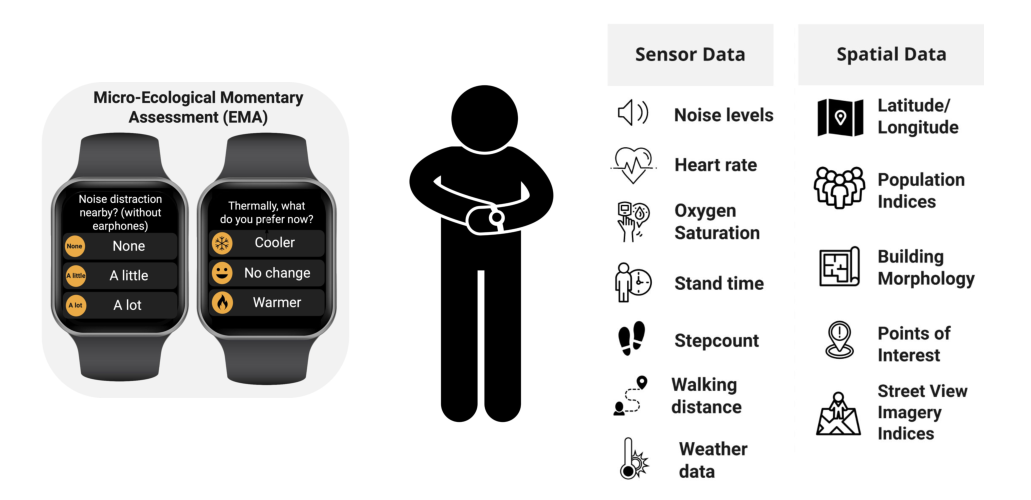
\includegraphics[width=0.92\textwidth]{figures/methods/cozie_study_design.pdf}
\caption{[PLACEHOLDER: Study design and data-collection workflow.]}
\label{fig:cozie-study-design}
\end{figure}

[PLACEHOLDER: Describe the derived survey-level dataset
(\texttt{cozie\_sg\_surveys\_with\_health\_aggregates}): 9{,}962 responses,
106 participants, 99+ columns. Explain how HealthKit physiological metrics are
aggregated to a 1-hour pre-survey window and how home locations were recovered.]

\subsubsection{Micro-survey structure}\label{sec:methods-perception}
[PLACEHOLDER: List subjective variables --- thermal preference, noise level,
noise kind, earphones, social context (alone/group), activity --- and their
response categories.]

\begin{figure}[htbp]
\centering
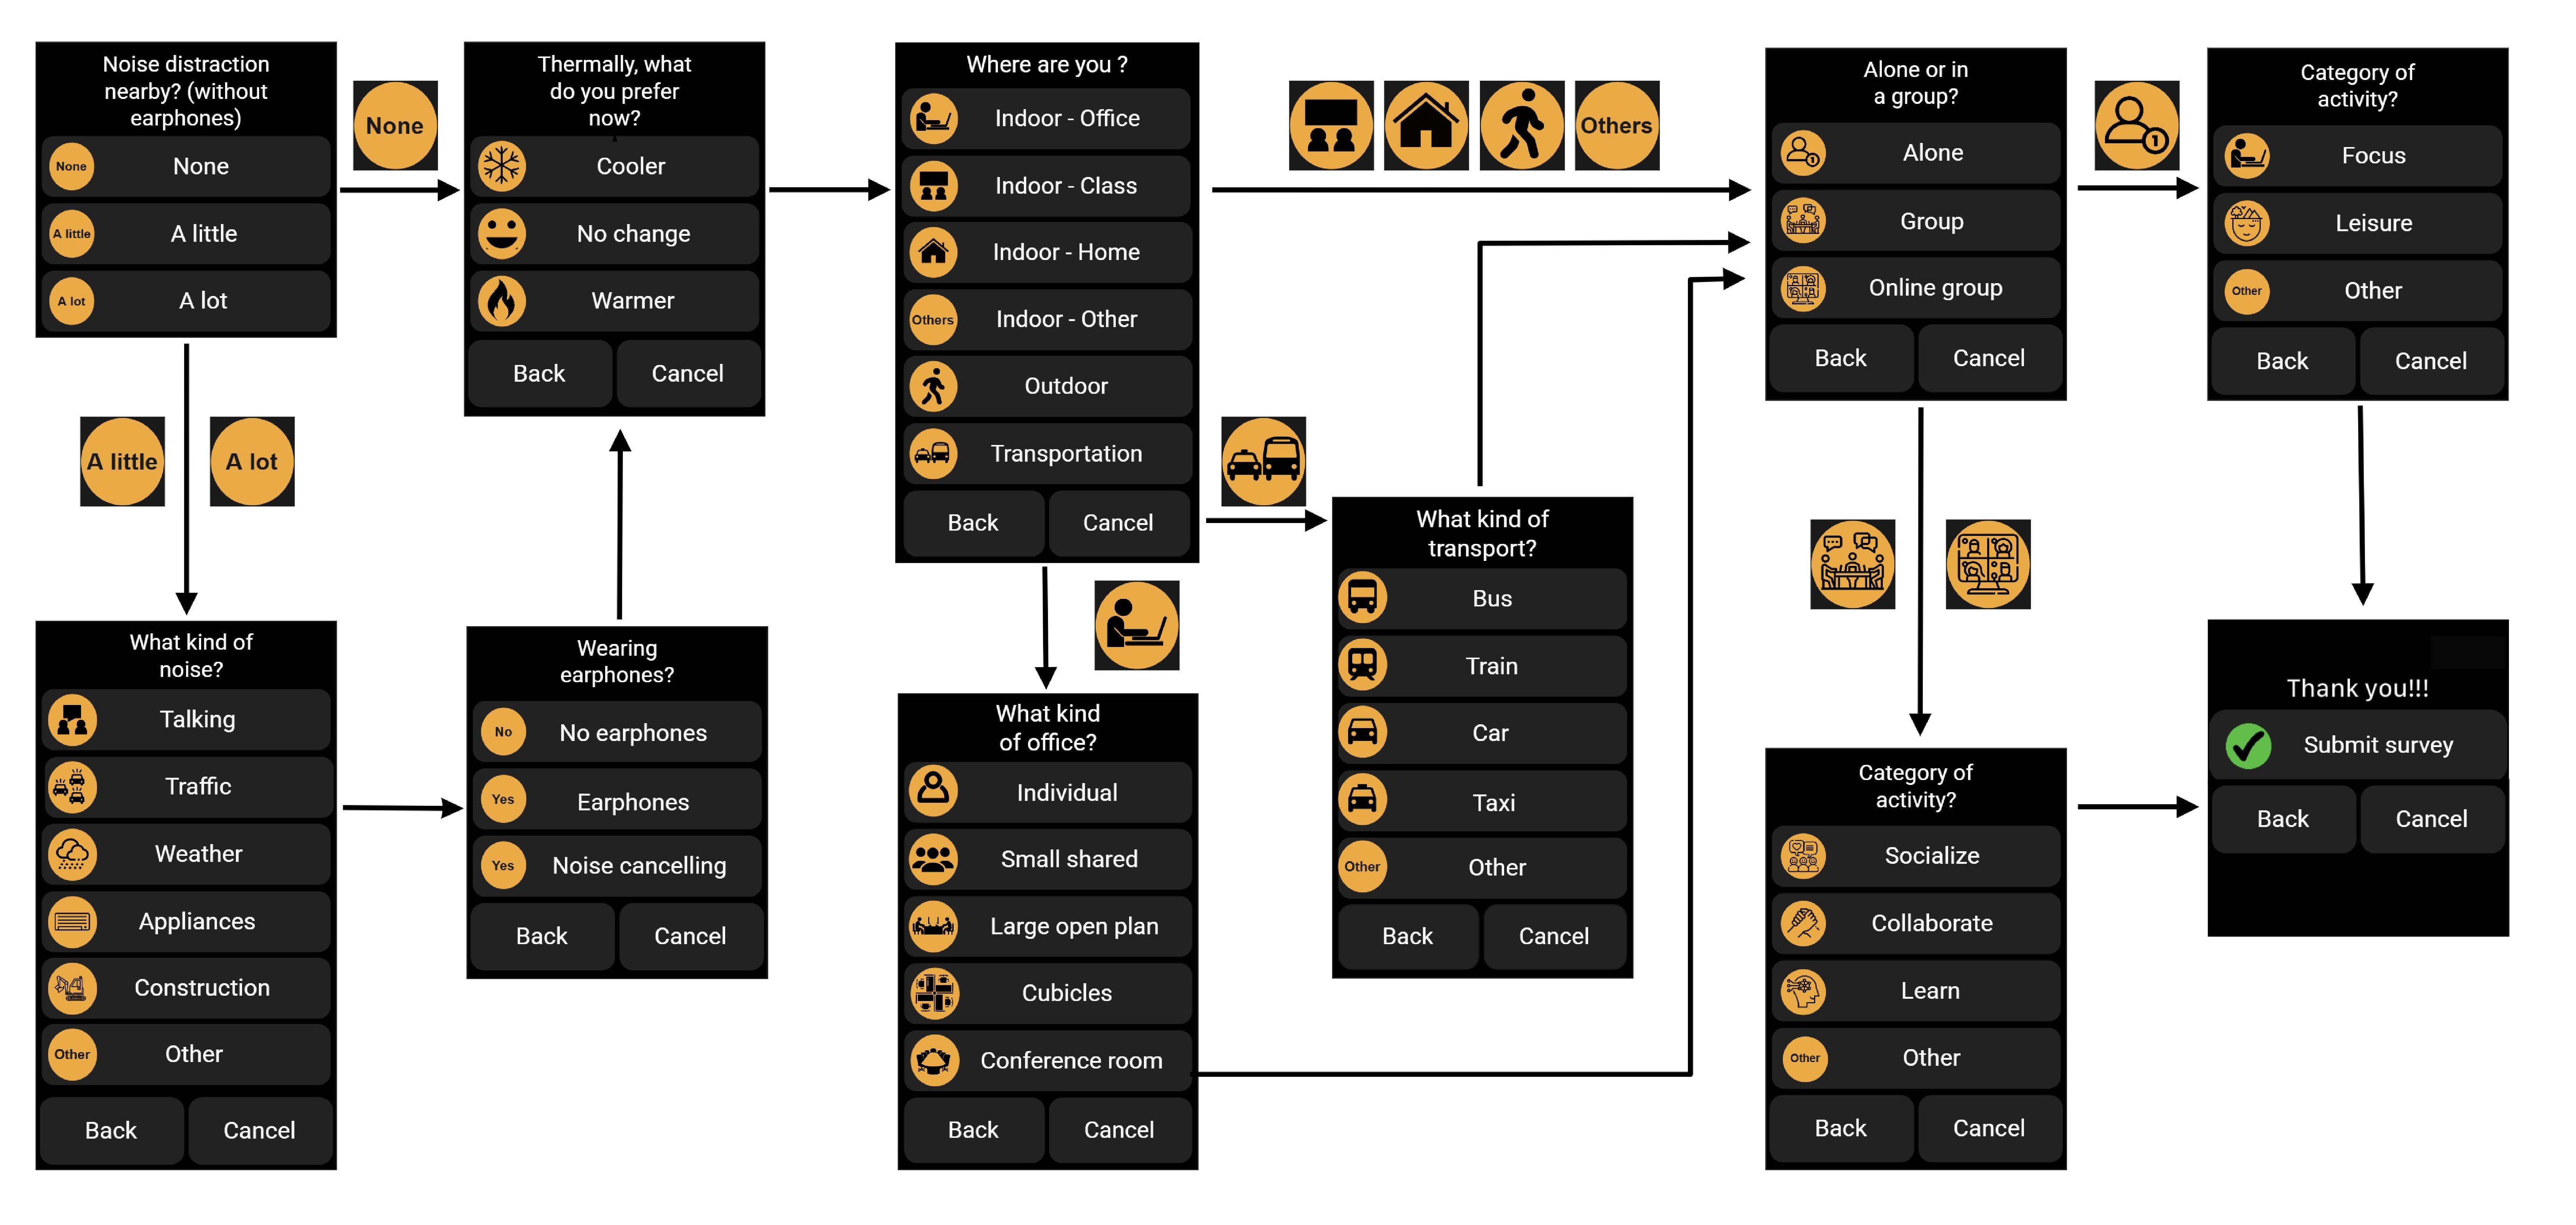
\includegraphics[width=0.92\textwidth]{figures/methods/cozie_microsurvey.pdf}
\caption{[PLACEHOLDER: Cozie smartwatch micro-survey interface and response flow.]}
\label{fig:cozie-microsurvey}
\end{figure}

[PLACEHOLDER: Describe 1-hour aggregates --- mean heart rate, total steps,
walking distance.]

% \subsubsection{Urban contextual indicators using Urbanity}\label{sec:methods-urbanform}
% [PLACEHOLDER: Describe geolocated environmental features --- green/sky/building/
% road view, visual complexity, building count, population, POI categories.]

\subsubsection{Weather data}\label{sec:methods-weather}
[PLACEHOLDER: Describe the nearest-station weather aggregation --- air
temperature, relative humidity, heat index, wind speed, rain, is-raining flag ---
units and coverage (92--96\%). Note this is ambient, not skin-level, exposure.]


\subsection{Data processing and characterization}\label{sec:methods-eda}
[PLACEHOLDER: Describe the EDA strategy from notebook 01 --- univariate survey /
health distributions, thermal relationships, temporal profiling in Singapore
local time, and geospatial mapping.]

[PLACEHOLDER: Describe the characterization methods from notebook 03 ---
perception fingerprints (row-normalized conditional proportions and lift),
association and effect size (Kruskal--Wallis $\varepsilon^2$, chi-square /
Cram\'er's V, Spearman $\rho$), and multivariate structure (MCA + k-modes
clustering).]


[PLACEHOLDER: Describe how weather features augment the characterization and the
direct test of whether thermal preference tracks actual heat index / rain.]

[PLACEHOLDER: Describe the space-type classifier (features = perceptions
$\pm$ weather), validation, and importance / SHAP attribution.]


% ============================================================================
\section{Results}\label{sec:results}
% ============================================================================

\subsection{Dataset overview and survey responses}\label{sec:res-overview}
[PLACEHOLDER: Summarize the dataset and headline distributions of survey
responses and health metrics.]

\begin{figure}[htbp]
\centering
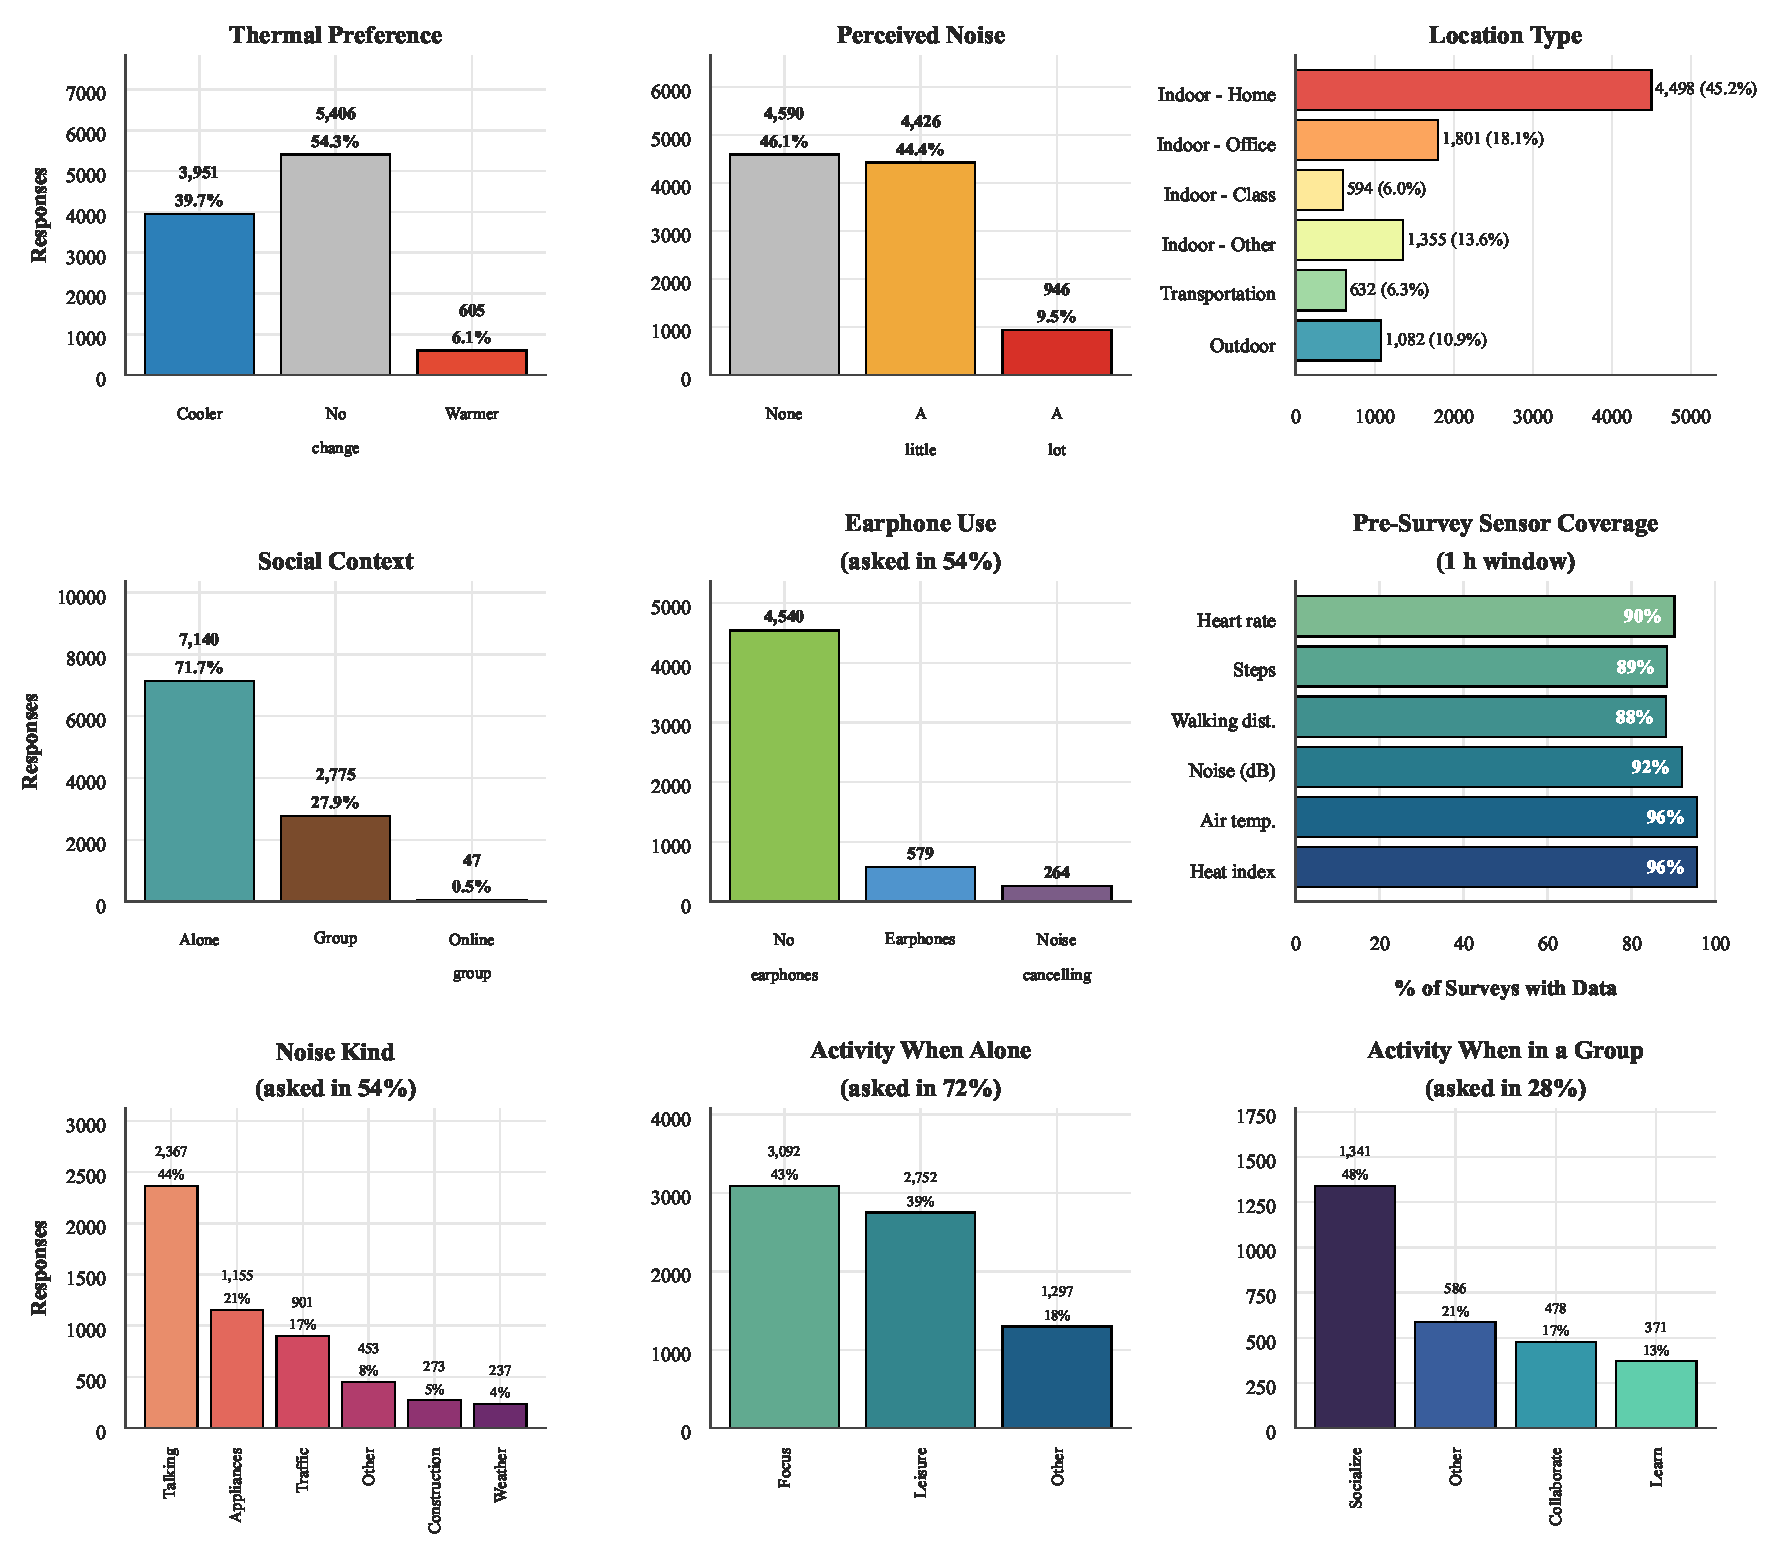
\includegraphics[width=\textwidth]{figures/data_characterization/survey_battery_and_coverage.pdf}
\caption{[PLACEHOLDER: Survey response battery, conditional follow-ups, and linked-sensor coverage (Figure A1).]}
\label{fig:data-a1-survey-battery}
\end{figure}

[PLACEHOLDER: Describe the survey response-flow structure.]

\begin{figure}[htbp]
\centering
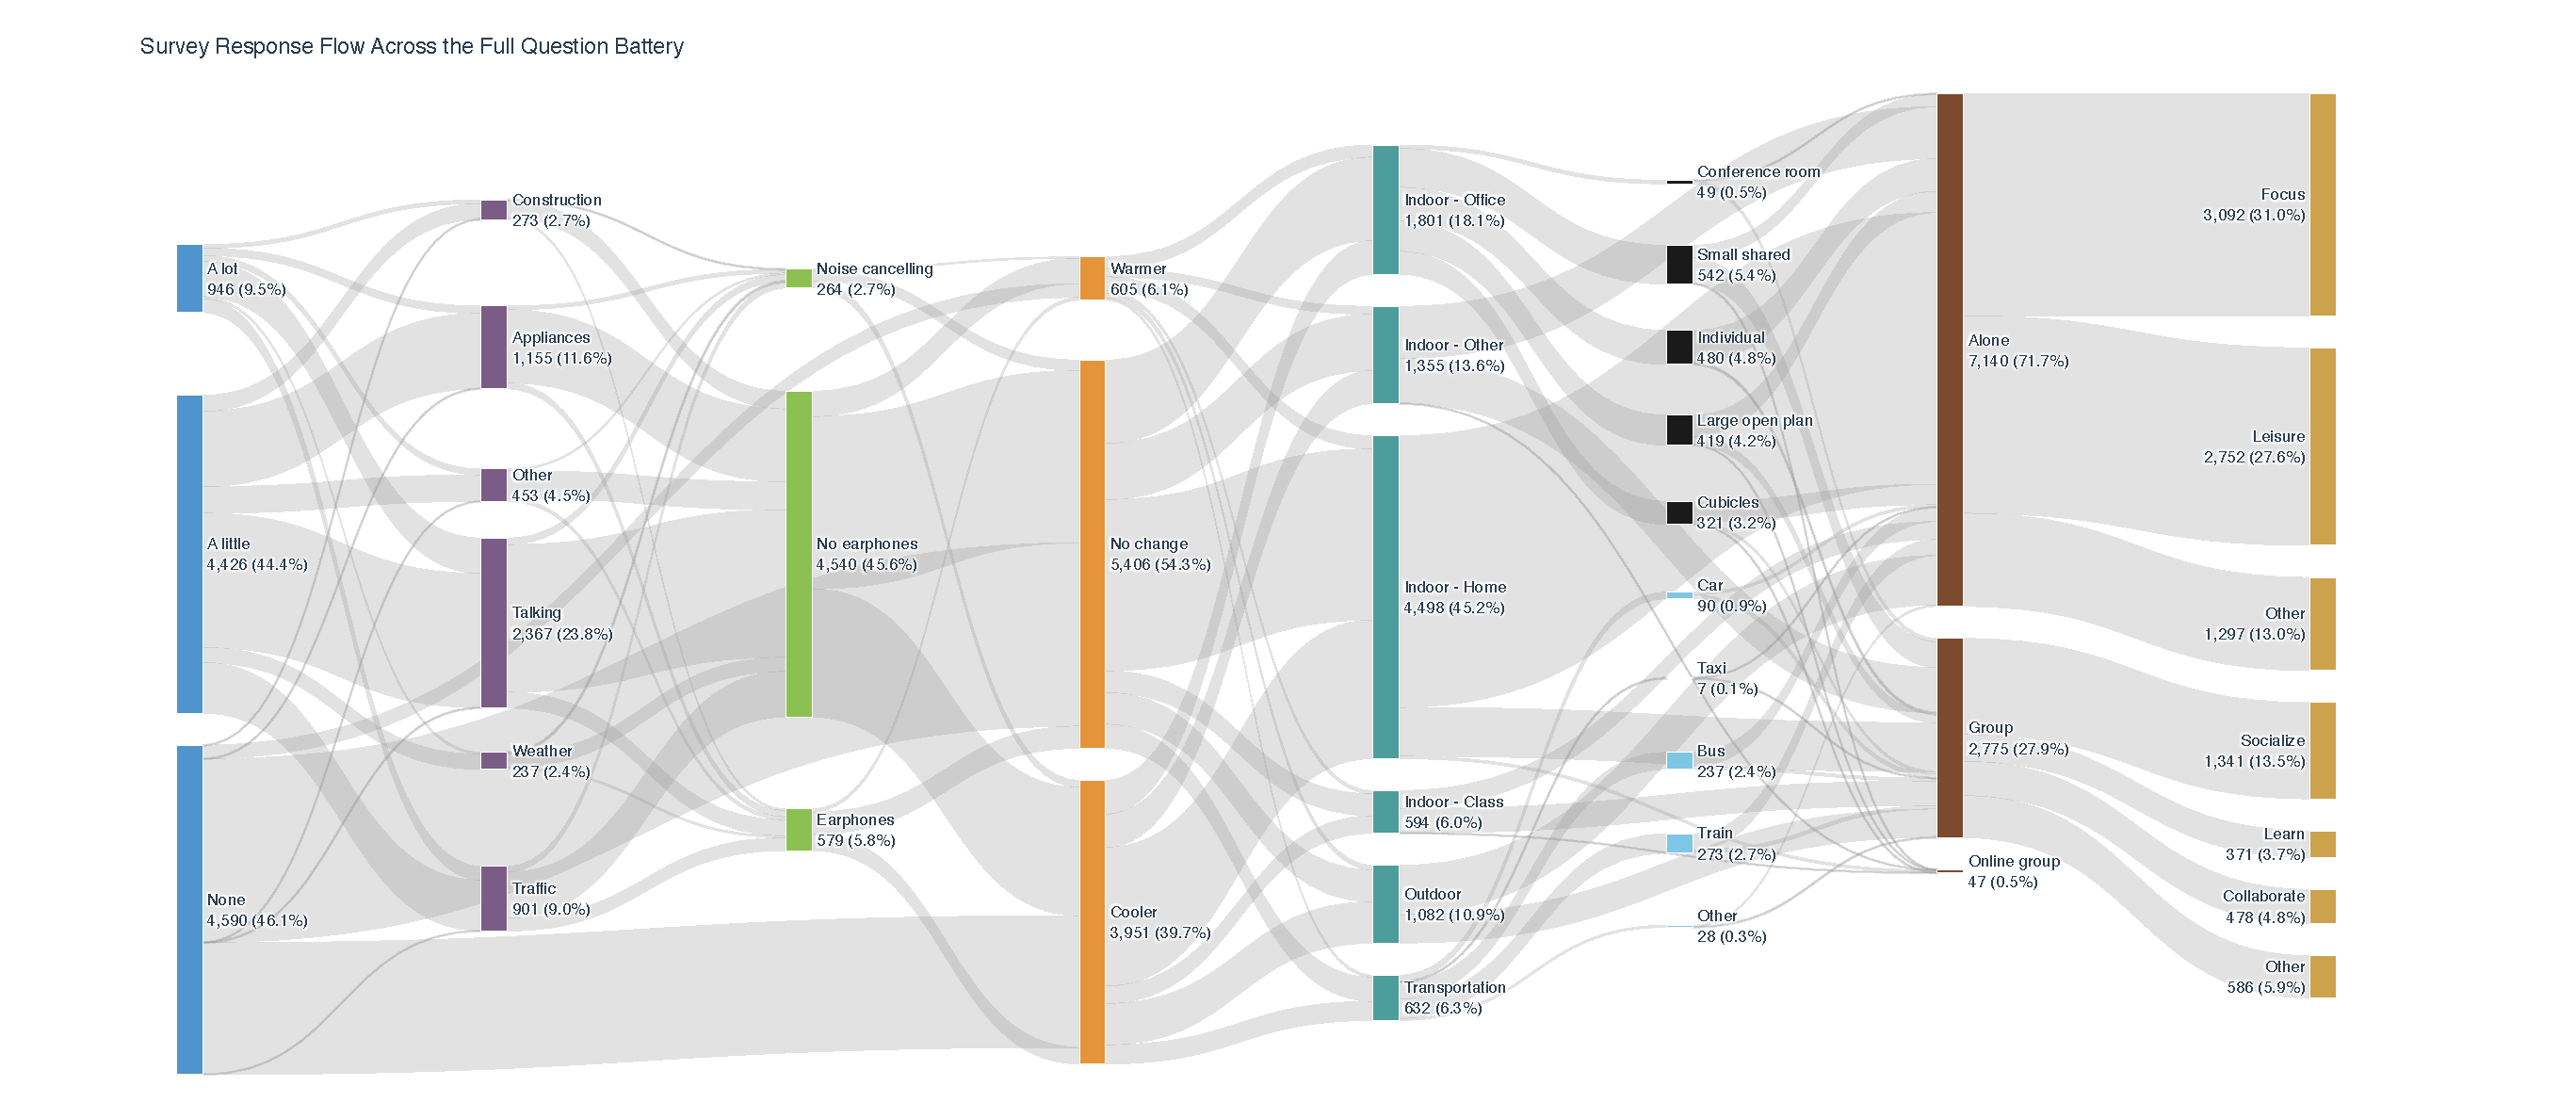
\includegraphics[width=\textwidth]{figures/data_characterization/survey_response_flow.pdf}
\caption{[PLACEHOLDER: Conditional response flow through the watch-survey questionnaire.]}
\label{fig:survey-response-flow}
\end{figure}


[PLACEHOLDER: Describe the island-wide geospatial patterns --- response density,
spatial thermal preference, green-view exposure, heart-rate hotspots, and the
per-space-type density facets.]

\begin{figure}[htbp]
\centering
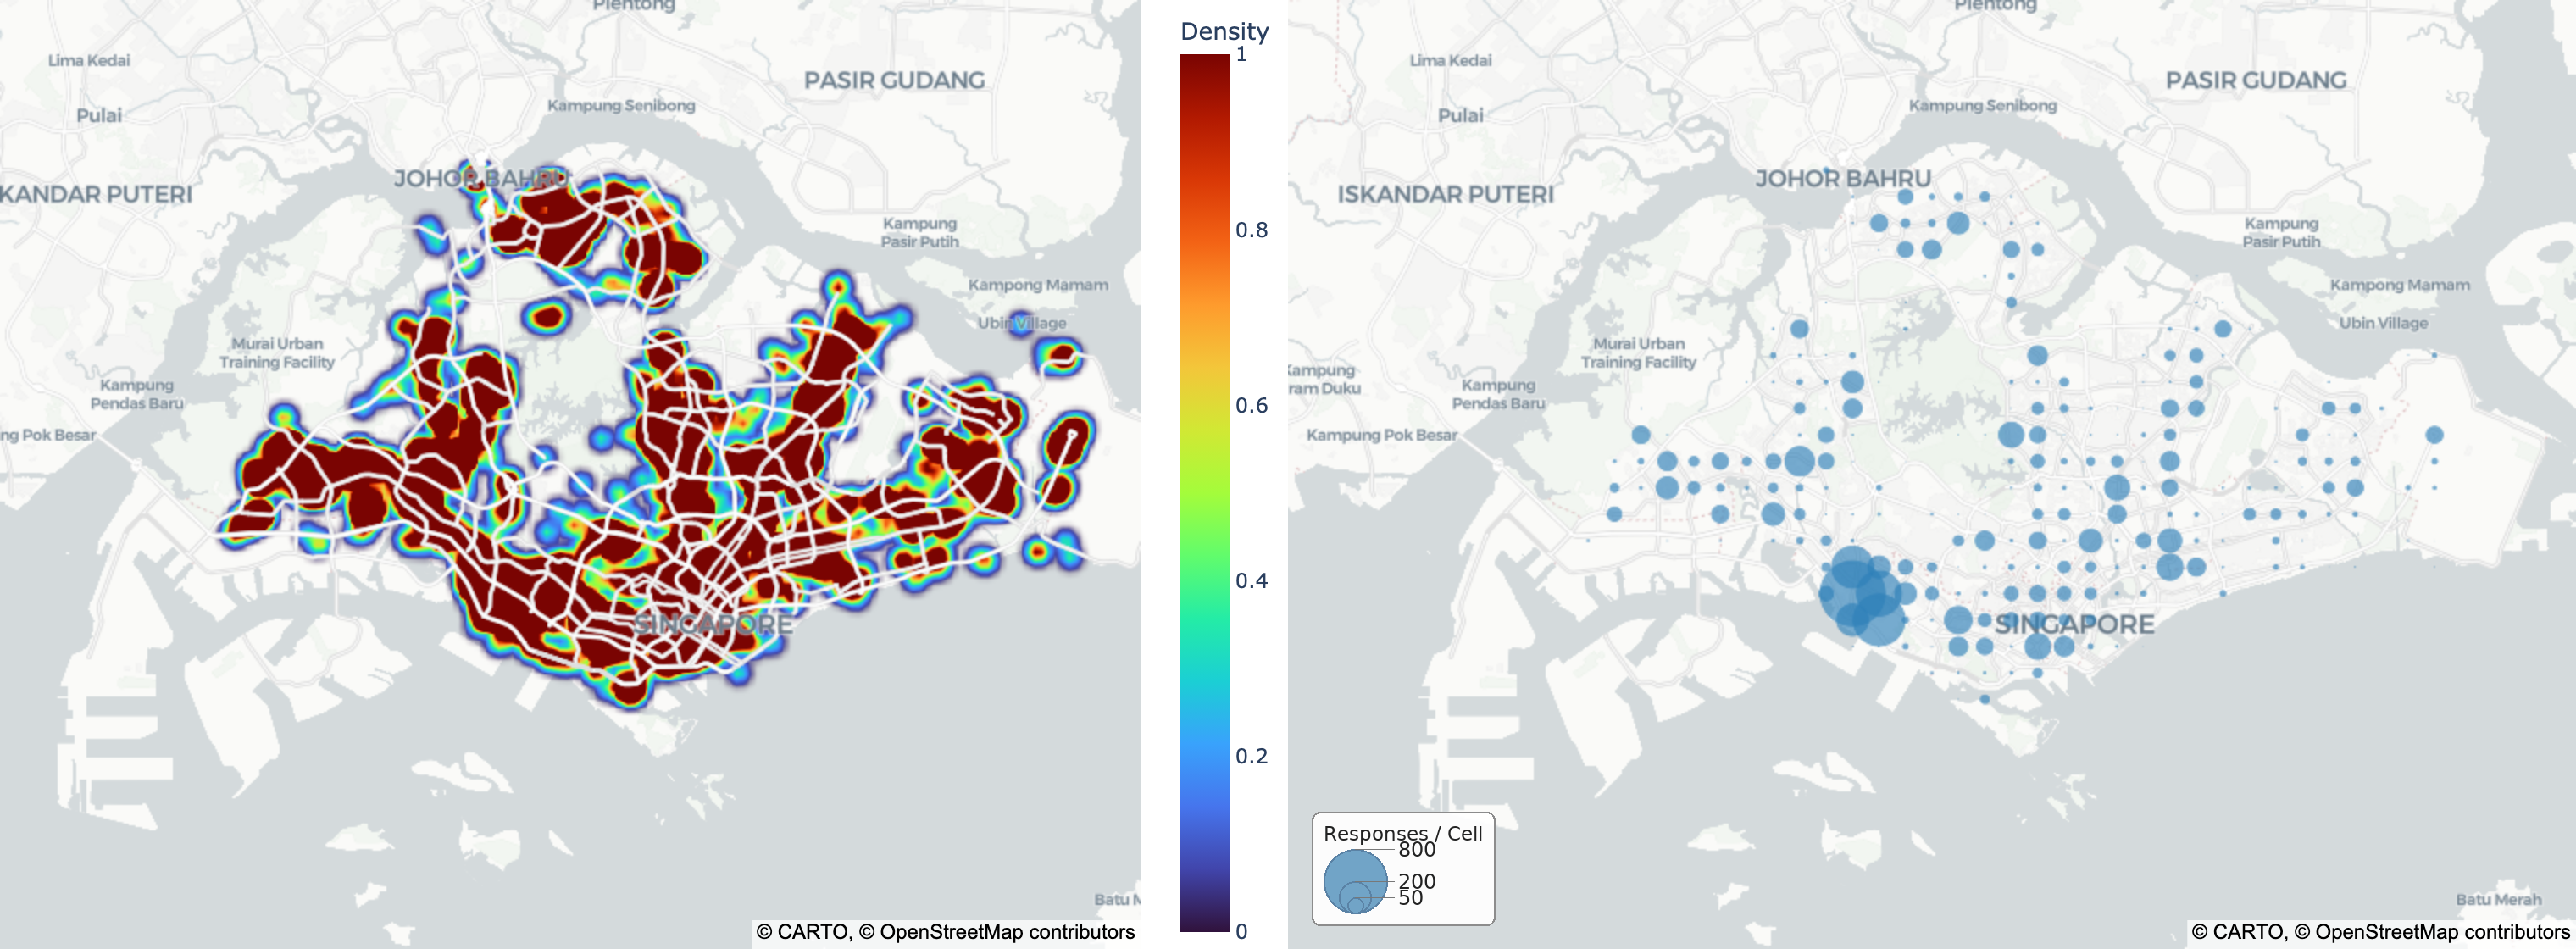
\includegraphics[width=\textwidth]{figures/data_characterization/response_density_and_grid_counts.png}
\caption{[PLACEHOLDER: Survey-response density and response counts by approximately 1-km grid cell across Singapore (Figure B4).]}
\label{fig:data-b4-response-density-grid-counts}
\end{figure}

\begin{figure}[htbp]
\centering
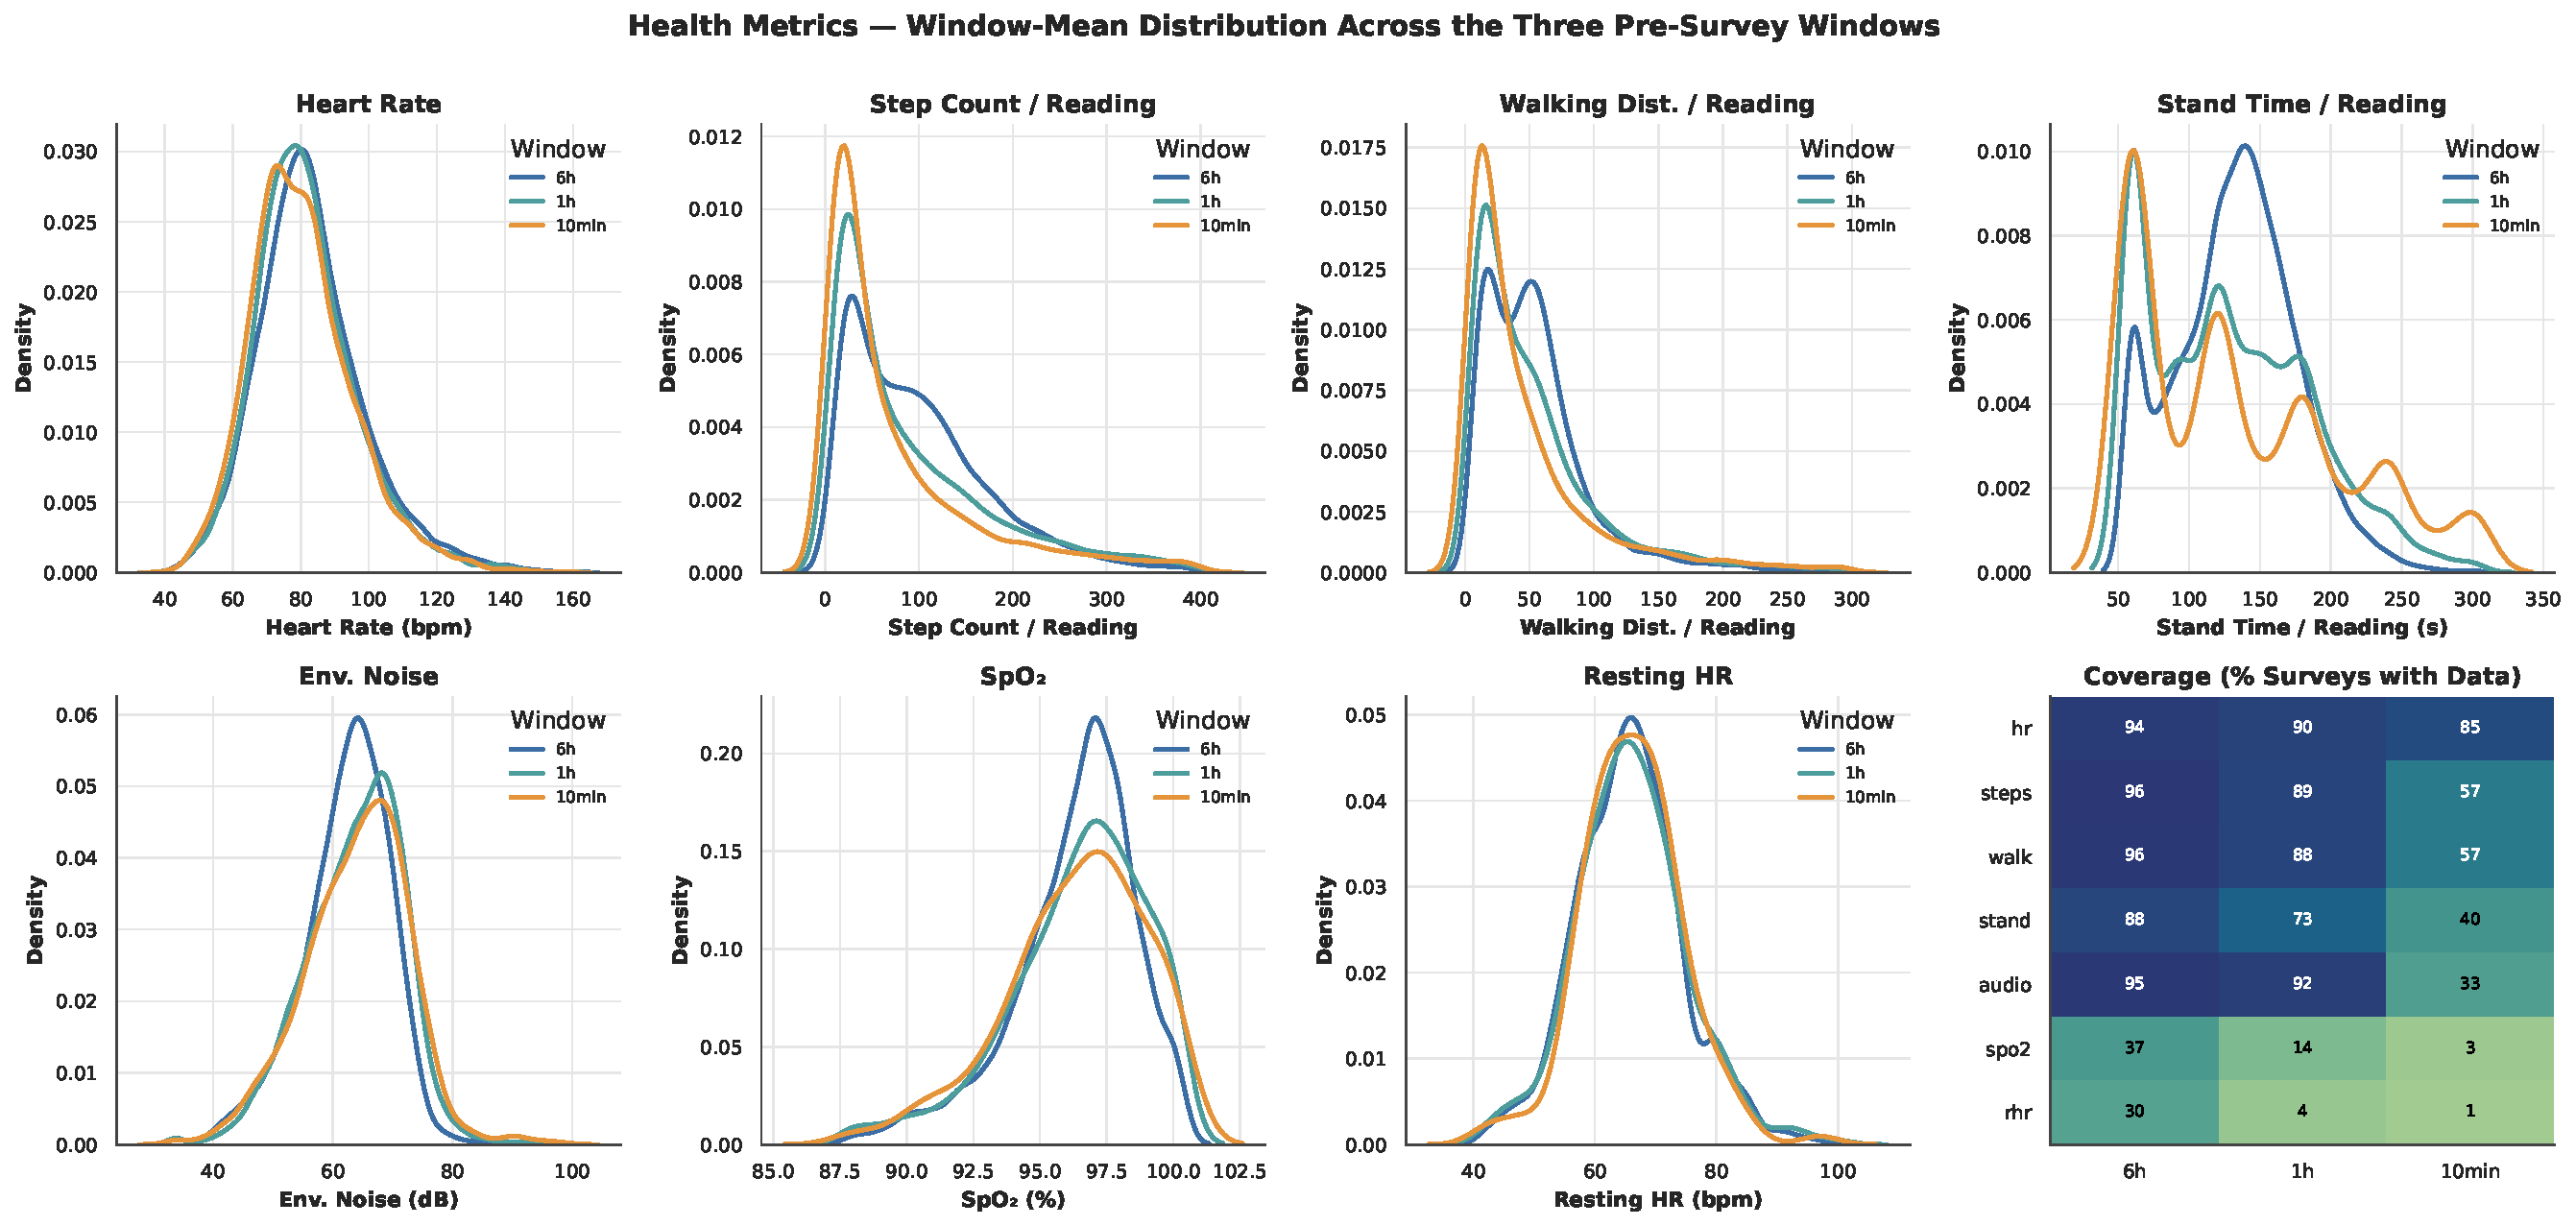
\includegraphics[width=\textwidth]{figures/data_characterization/wearable_health_windows.pdf}
\caption{[PLACEHOLDER: Wearable-health metrics across pre-survey aggregation windows (Figure A2).]}
\label{fig:data-a2-health-windows}
\end{figure}

\begin{figure}[htbp]
\centering
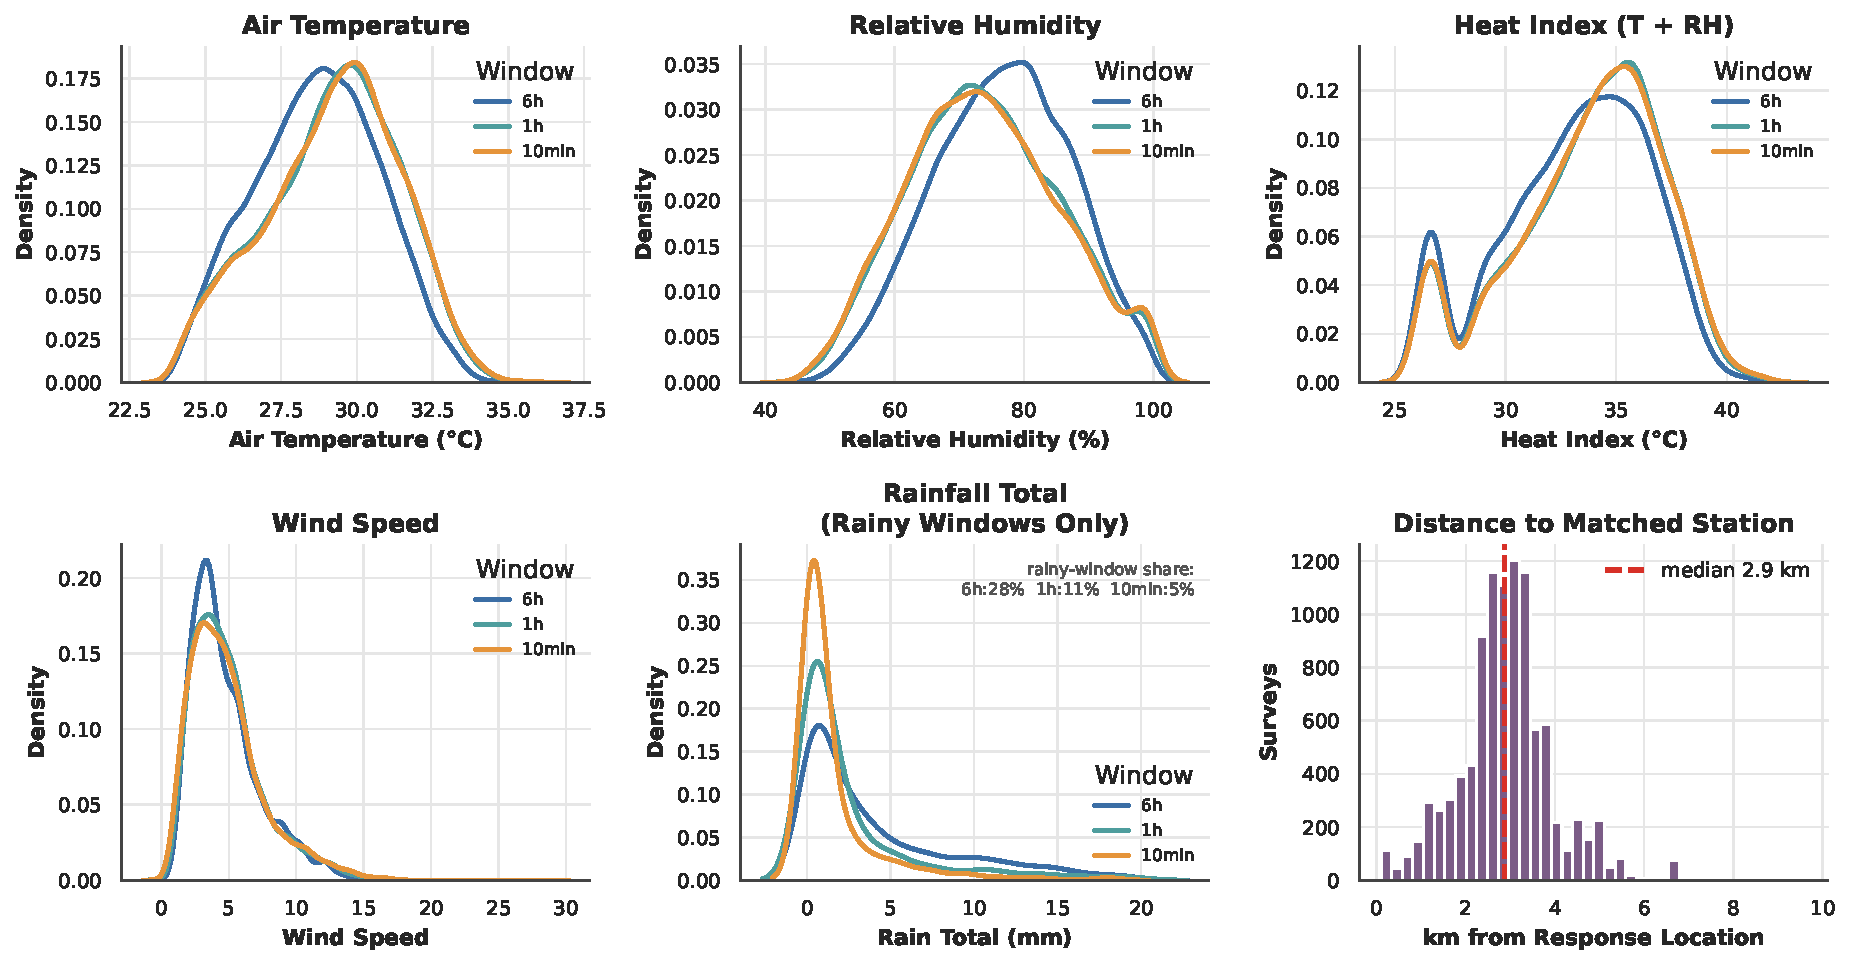
\includegraphics[width=\textwidth]{figures/data_characterization/outdoor_weather_windows.pdf}
\caption{[PLACEHOLDER: Nearest-station outdoor ambient weather across pre-survey aggregation windows (Figure A3).]}
\label{fig:data-a3-weather-windows}
\end{figure}


\subsection{Temporal patterns of response submission}\label{sec:res-temporal}
[PLACEHOLDER: Describe when surveys are filled out (Singapore local time) and how
timing is strongly space-type dependent (Office/Classroom weekday-afternoon vs
Home evening/weekend vs bimodal Transportation).]

\begin{figure}[htbp]
\centering
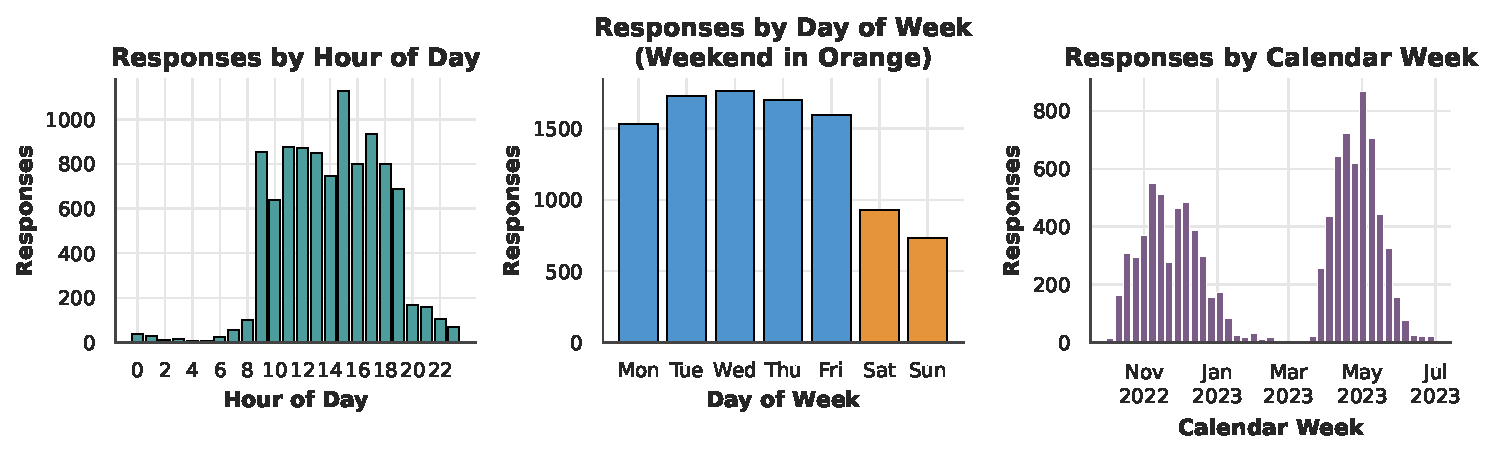
\includegraphics[width=\textwidth]{figures/data_characterization/weekly_temporal_cadence.pdf}
\caption{[PLACEHOLDER: Weekly temporal cadence of survey responses in Singapore local time (Figure D2).]}
\label{fig:data-d2-temporal-cadence}
\end{figure}

\begin{figure}[htbp]
\centering
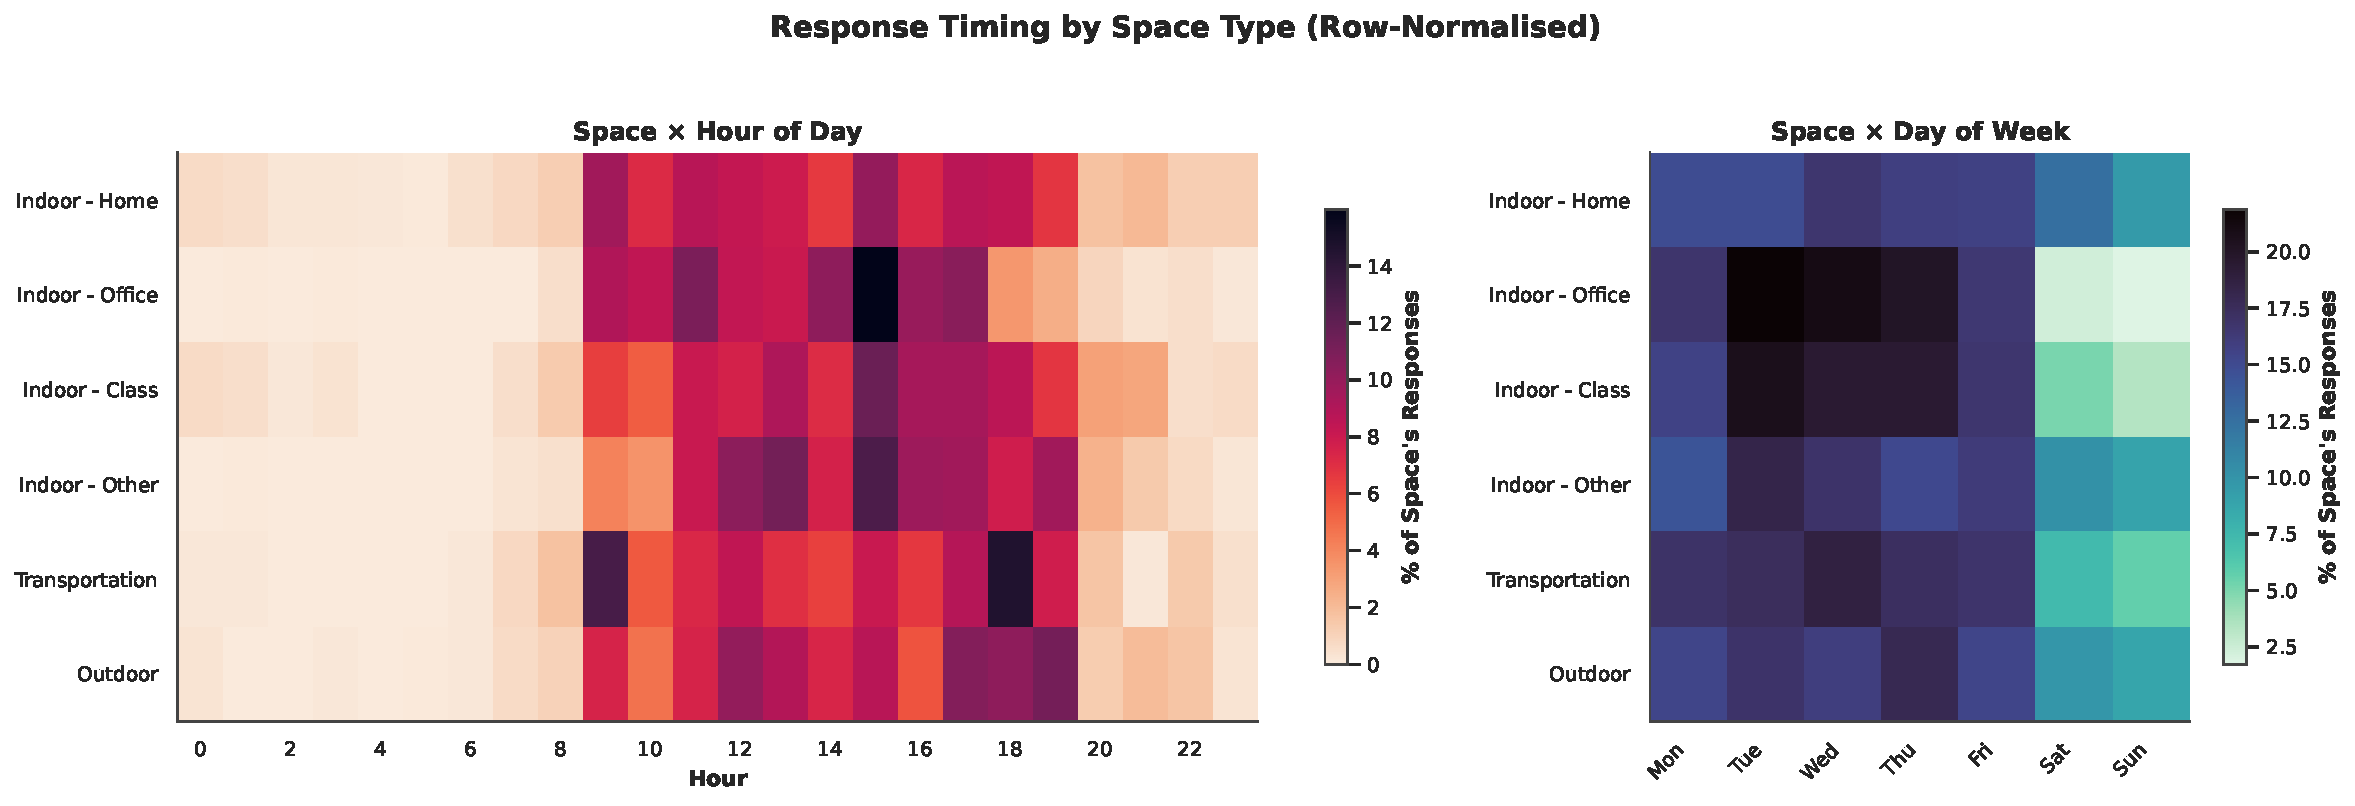
\includegraphics[width=\textwidth]{figures/data_characterization/space_type_timing_heatmaps.pdf}
\caption{[PLACEHOLDER: Response timing by space type, shown by hour of day and day of week (Figure D4).]}
\label{fig:data-d4-space-time}
\end{figure}

\subsection{Per-participant heterogeneity}\label{sec:res-participant}
[PLACEHOLDER: Describe between-participant variation in space-type / perception
shares (stacked bars and distribution-of-shares histograms).]

\begin{figure}[htbp]
\centering
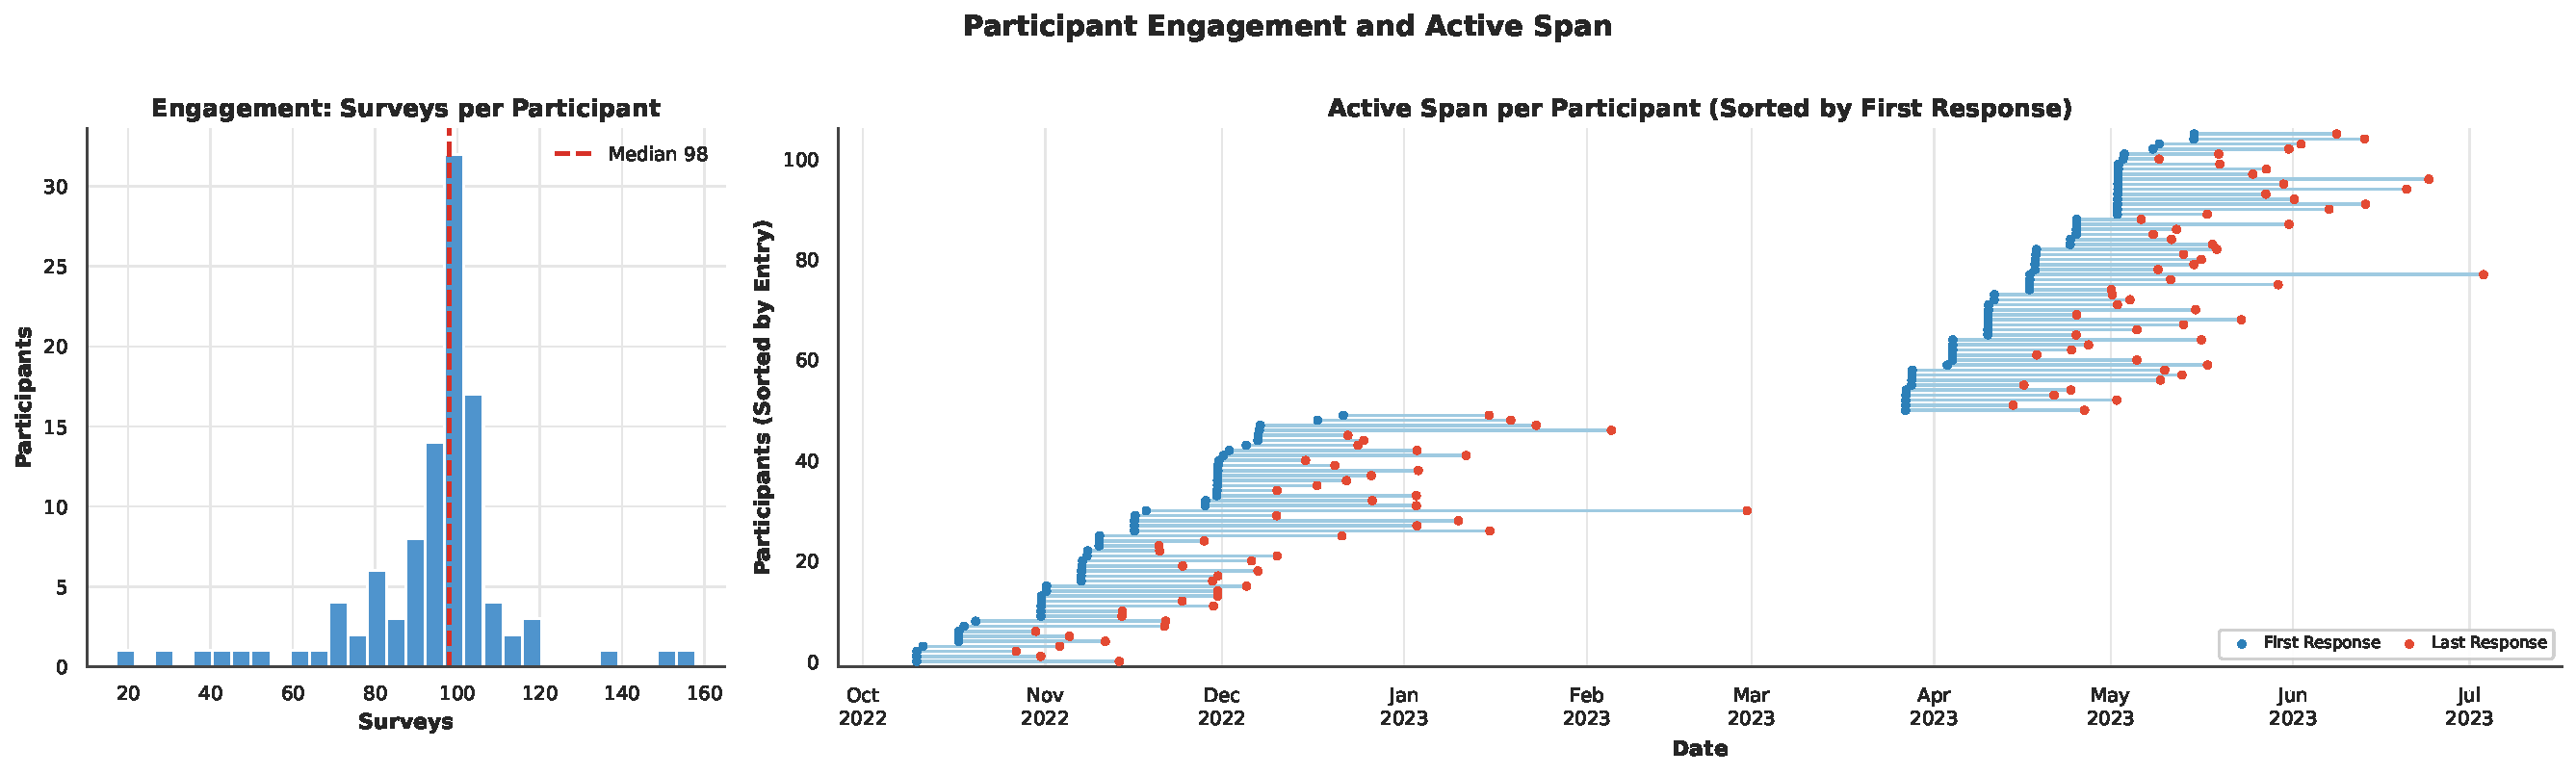
\includegraphics[width=\textwidth]{figures/data_characterization/participant_engagement.pdf}
\caption{[PLACEHOLDER: Participant engagement and active survey span (Figure E2).]}
\label{fig:data-e2-engagement}
\end{figure}

\subsection{Cooling preference}\label{sec:res-cooling}

\begin{figure}[htbp]
\centering
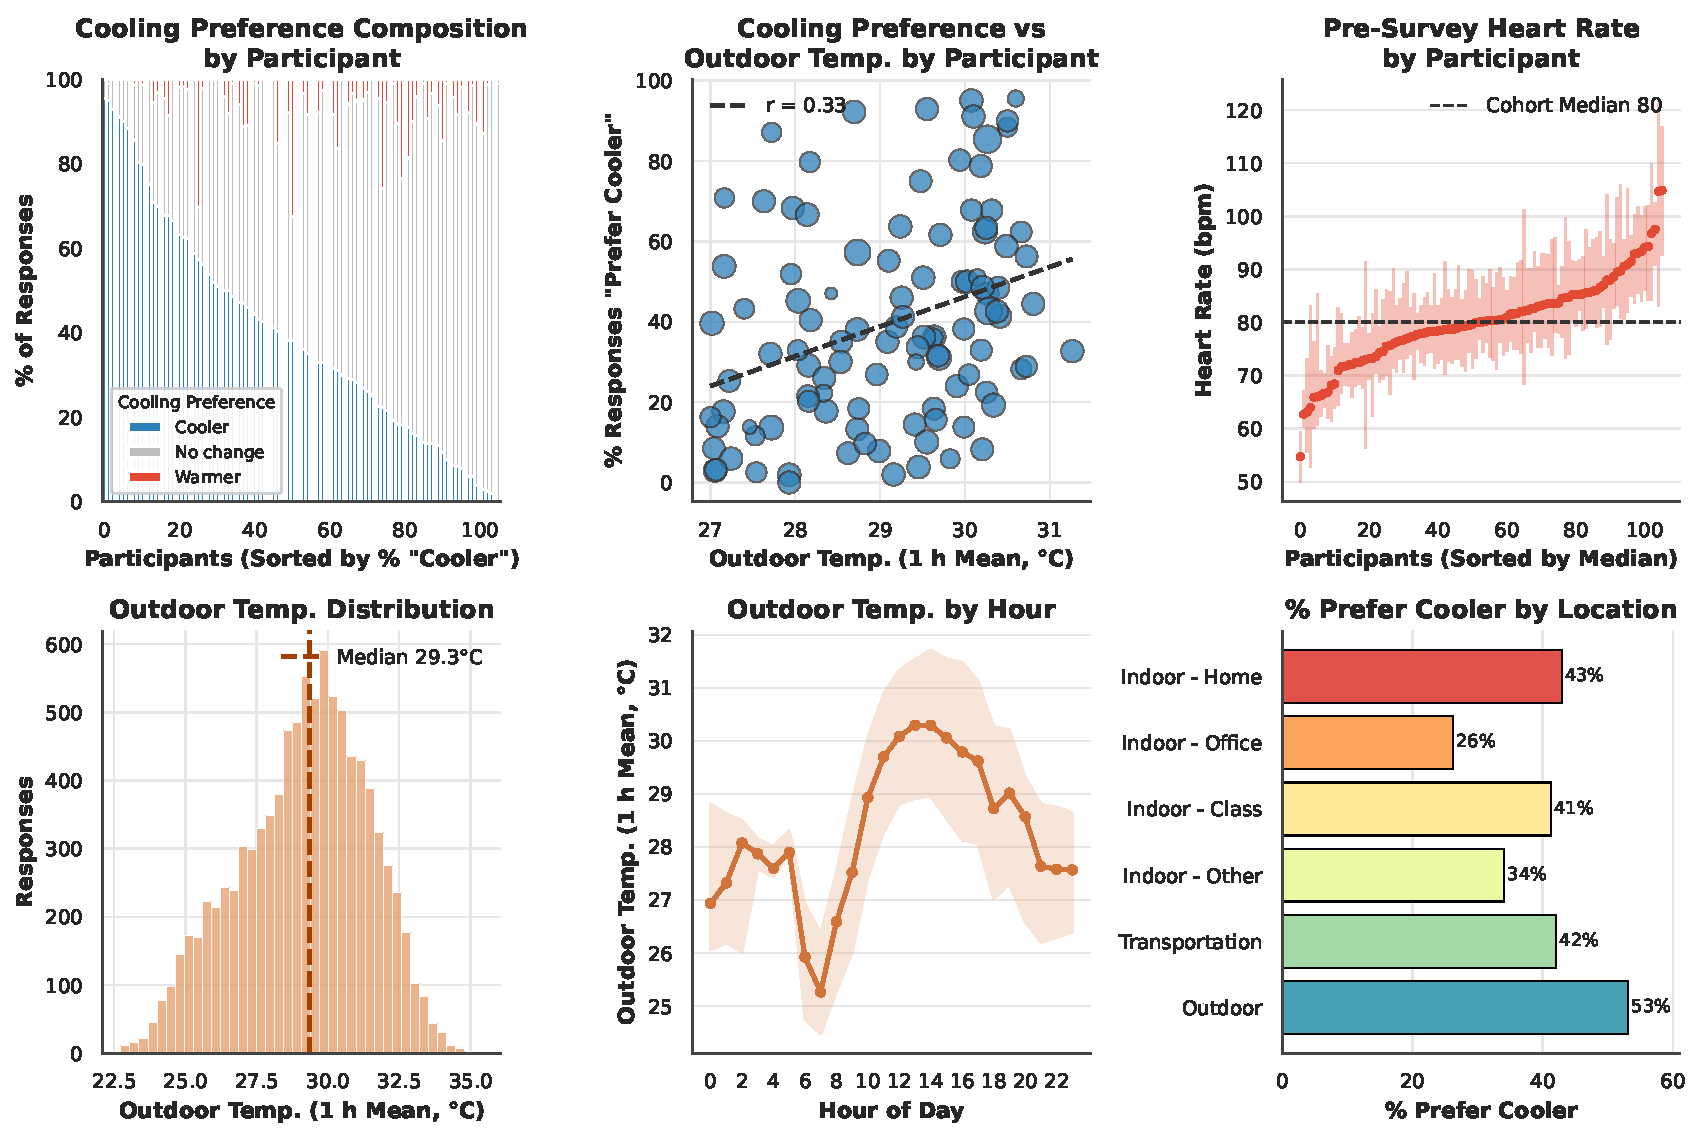
\includegraphics[width=\textwidth]{figures/data_characterization/cooling_preference.pdf}
\caption{[PLACEHOLDER: Participant-level and contextual patterns in cooling preference (Figure F2).]}
\label{fig:data-f2-cooling}
\end{figure}

\subsection{Noise preference}\label{sec:res-noise}

% The source notebook identifies this visualization as Figure G1 (not G2).
\begin{figure}[htbp]
\centering
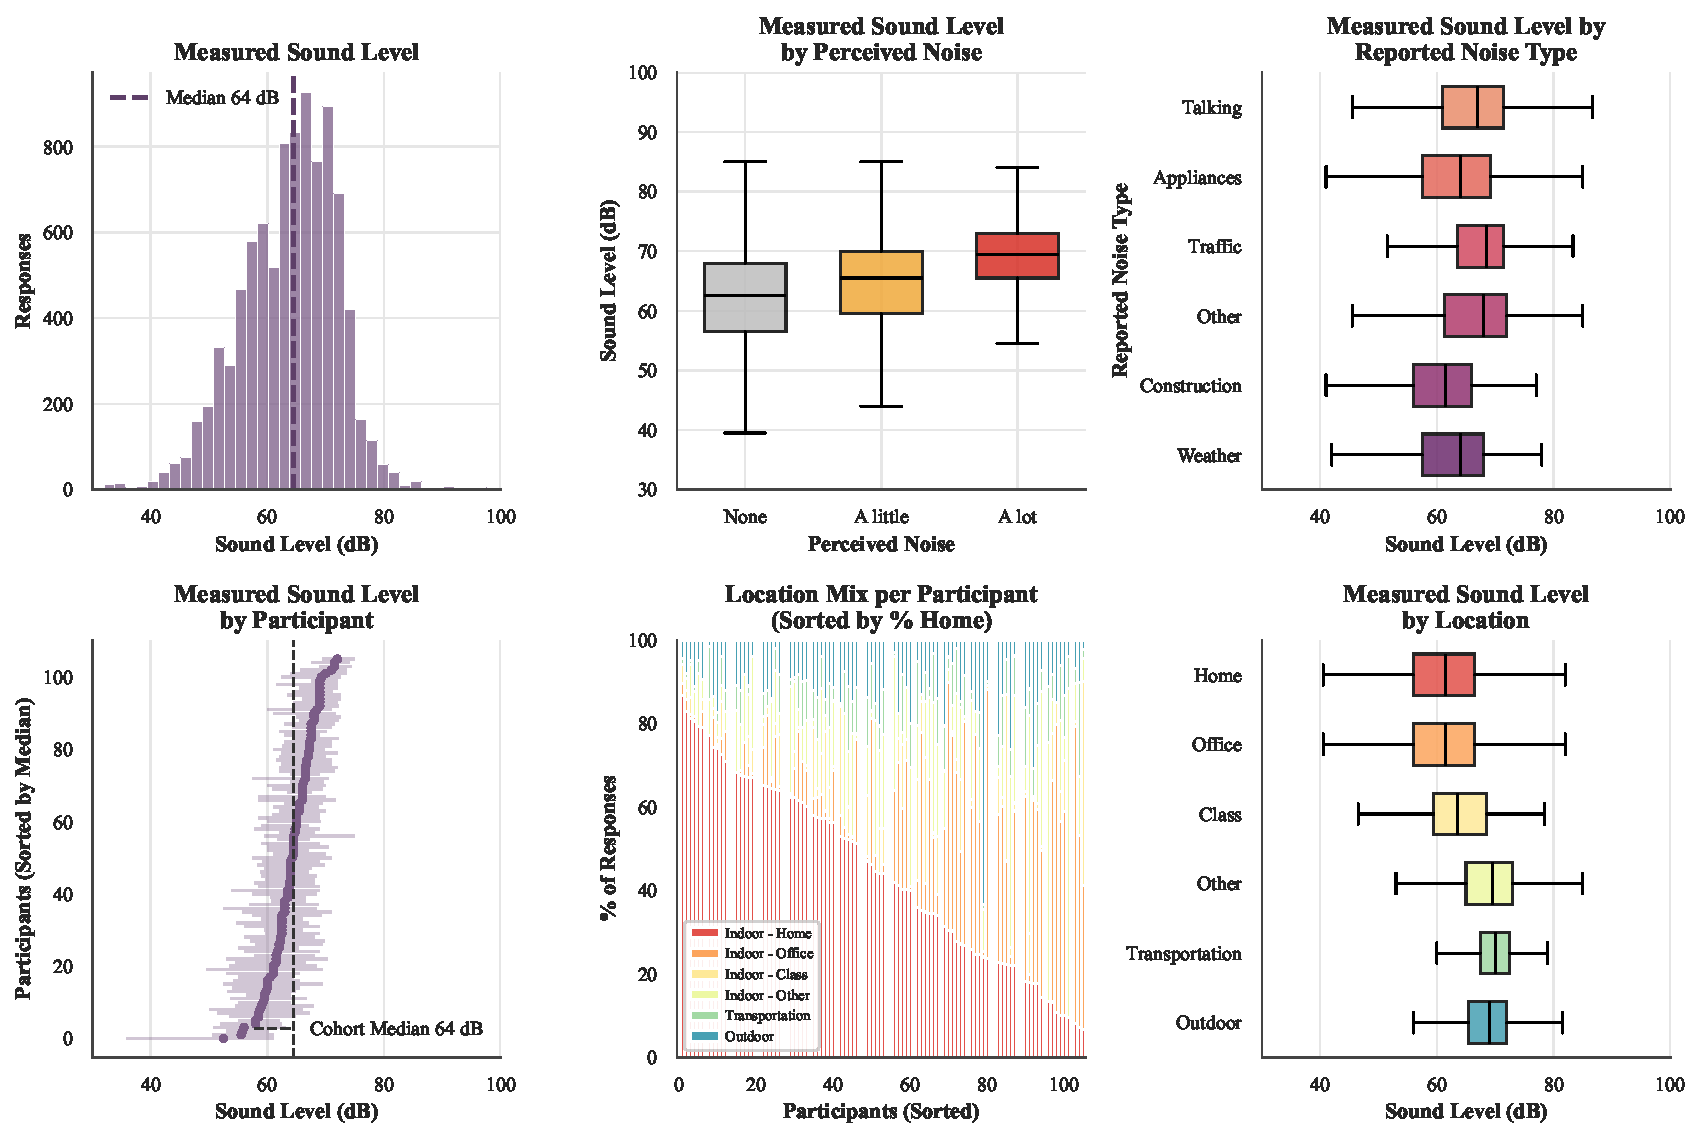
\includegraphics[width=\textwidth]{figures/data_characterization/noise_characterization.pdf}
\caption{[PLACEHOLDER: Measured sound level across subjective, participant, and location contexts (Figure G1).]}
\label{fig:data-g1-noise}
\end{figure}


\subsection{Perceptual fingerprints by space type}\label{sec:res-fingerprint}
[PLACEHOLDER: Describe the perception fingerprint (P(response$\mid$space)) and the
lift table flagging distinctive perceptions per space type.]


\subsection{Statistical association and effect size}\label{sec:res-association}
[PLACEHOLDER: Report association strength between space type and each
perceptual variable (Cram\'er's V), emphasizing effect sizes over p-values.]


\subsection{Multivariate structure of experience}\label{sec:res-mca}
[PLACEHOLDER: Describe MCA + k-modes clustering of the subjective experience and
how clusters relate (or not) to space type.]

\subsection{Physiological and weather signatures}\label{sec:res-physio-weather}
[PLACEHOLDER: Report physiological gradient across spaces (sedentary Home to
mobile Outdoor/Transport; steps largest effect) and the weak ambient-weather
signatures --- ambient weather barely marks space type; Outdoor is not the
hottest.]

\subsection{Weather versus thermal preference}\label{sec:res-weather-tp}
[PLACEHOLDER: Report the key new result --- ``Cooler'' responses occur in
genuinely hotter (higher heat-index) and drier conditions; rain suppresses
cooling demand. Effect is real but modest.]


\subsection{Outdoor environmental characterization}\label{sec:res-outdoor}
[PLACEHOLDER: Restricted to Outdoor responses --- streetscape/built-form profile,
its (weak) link to thermal preference, environment--physiology nulls, and actual
weather vs outdoor thermal preference.]



\subsection{Discriminative modeling of space type}\label{sec:res-model}
[PLACEHOLDER: Report the space-type classifier performance and feature importance
(activity and noise-kind as strong space descriptors; ambient weather adds little).]


% ============================================================================
\section{Discussion}\label{sec:discussion}
% ============================================================================

\subsection{Principal findings}\label{sec:disc-findings}
[PLACEHOLDER: Synthesize: function/behaviour (activity, noise + coping, movement)
separates space types robustly; thermal, environmental and physiological
expectations are mostly weak or convergent nulls; the weather correction shows
ambient weather is nearly useless for identifying a space yet genuinely drives
outdoor thermal preference.]

\subsection{Interpretation against intuition}\label{sec:disc-intuition}
[PLACEHOLDER: Discuss the reinforced vs contradicted intuitions (e.g. Outdoor is
not the hottest; streetscape greenery does not move thermal preference; actual
heat does).]

\subsection{Implications for sustainable urban design}\label{sec:disc-implications}
[PLACEHOLDER: Connect findings to the journal scope --- what they mean for
thermal-comfort-aware, health-supportive and energy-conscious urban design and
policy in tropical cities.]

\subsection{Limitations}\label{sec:disc-limitations}
[PLACEHOLDER: Participant nesting / pseudoreplication; ambient nearest-station
weather as a coarse proxy for personal exposure; convenience sample; Singapore-
specific A/C context; self-reported perceptions.]

\subsection{Future work}\label{sec:disc-future}
[PLACEHOLDER: Directions --- personal microclimate sensing, larger/more diverse
cohorts, cross-city replication, mixed-effects modeling accounting for
participant nesting.]


% ============================================================================
\section{Conclusion}\label{sec:conclusion}
% ============================================================================
[PLACEHOLDER: Concise restatement of the contribution and headline takeaway for
sustainable urban development.]


% ============================================================================
\section*{Acknowledgements}
% ============================================================================
[PLACEHOLDER: Acknowledgements.]

\section*{Disclosure statement}
[PLACEHOLDER: Declare any competing interests.]

\section*{Funding}
[PLACEHOLDER: Funding sources.]

\section*{Data availability statement}
[PLACEHOLDER: Statement on ORENTH / Cozie-Singapore data availability.]


% ============================================================================
% References  (replace with your .bib and \bibliographystyle as required)
% ============================================================================
\bibliographystyle{apacite}% Taylor & Francis APA-style (matches the interact sample)
\bibliography{interactapasample}% [PLACEHOLDER: replace with your own .bib file]

\end{document}
